%% Demonstration of different definitions of interpolation.

\pgfplotsset{
    compat=1.5.1,
    oracle/.style={color=red, style=dashed, line width=1.5pt},
    objective/.style={color=black, style=solid, line width=1.5pt},
}

\tikzset{
    font={\fontsize{18pt}{12}\selectfont}},
}

\begin{figure}[]
    \centering
    \begin{tikzpicture}[scale=0.75, font size=50pt,
          declare function={
            objective(\x)=      (\x<=-1) * (2*\x*\x + 6*\x + 4)    +
            and(\x>-1, \x<=1) * (\x + 5 - pow(\x,3) - 5*\x*\x) / 4 +
                                (\x>1) * (\x*\x - 5*\x + 4); 
            oracle1(\x)=         (pow(\x - 2.5, 2) / 2 - 3.25);
          }
        ]
        \begin{axis}[
          axis x line=none, axis y line=none,
          ymin=-5, ymax=5, ytick={-5,...,5}, ylabel=$y$,
          xmin=-5, xmax=7, xtick={-5,...,7}, xlabel=$x$,
        ]
        \addplot[domain=-5:7, samples=100, objective]{objective(x)};
        \addplot[domain=-5:7, samples=100, oracle]{oracle1(x)};
        
        %% point labels
        \node[label={90:$\wopt$},circle,fill,inner sep=2pt] at (axis cs:2.5,-2.25) {};
        %% function labels
        \node[label={180:$f(\w)$}] at (axis cs:-2.4,2) {};
        \node[label={180:$f(\w, \z)$}] at (axis cs:1.25,-2.5) {};
        %% plot label
        \node[label={90:Minimizer}] at (axis cs:1,-5.2) {};
        \end{axis}
    \end{tikzpicture}%
    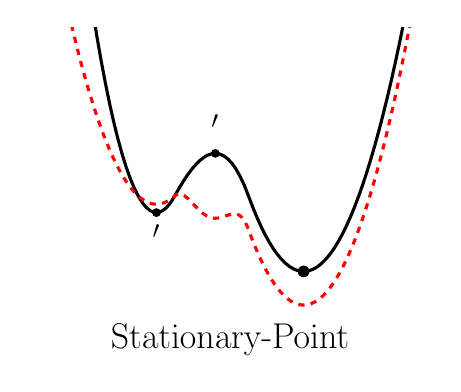
\begin{tikzpicture}[scale=0.75,
          declare function={
            objective(\x)=      (\x<=-1) * (2*\x*\x + 6*\x + 4)    +
            and(\x>-1, \x<=1) * (\x + 5 - pow(\x,3) - 5*\x*\x) / 4 +
                                (\x>1) * (\x*\x - 5*\x + 4); 
            oracle1(\x)=        (\x<=-1) * (pow(x + 1.5, 2))   +
            and(\x>-1, \x<=1) * (-305*pow(\x, 4)/264- 1*pow(\x, 3)/4 + 173*pow(\x,2)/132 - 1*\x/4 - 107/264) +
                                (\x>1) * (pow(x - 2.5, 2) - 3) - 0.25; 
          }
        ]
        \begin{axis}[
          axis x line=none, axis y line=none,
          ymin=-5, ymax=5, ytick={-5,...,5}, ylabel=$y$,
          xmin=-5, xmax=6, xtick={-5,...,6}, xlabel=$x$,
        ]
        \addplot[domain=-5:6, samples=100, objective]{objective(x)};
        \addplot[domain=-5:6, samples=200, oracle]{oracle1(x)};
        
        %% point labels
        \node[label={90:$\wopt$},circle,fill,inner sep=2pt] at (axis cs:2.5,-2.25) {};
        \node[label={90:$\w'$},circle,fill,inner sep=1.5pt] at (axis cs:0.1,1.262) {};
        \node[label={270:$\w'$},circle,fill,inner sep=1.5pt] at (axis cs:-1.5,-0.5) {};
        %% function labels
        %\node[label={0:$f(\w)$}] at (axis cs:-2.6,2.5) {};
        %\node[label={180:$f(\w, \z)$}] at (axis cs:1.25,-2.5) {};
        %% plot label
        \node[label={90:Stationary-Point}] at (axis cs:0.5,-5.2) {};
        \end{axis}
    \end{tikzpicture}%
    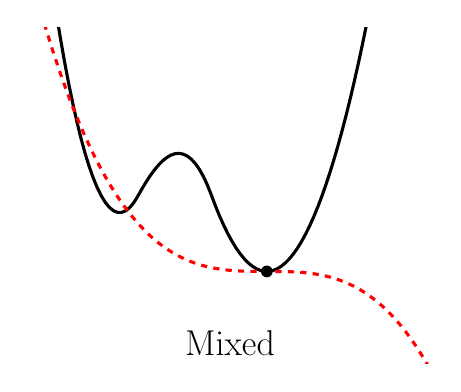
\begin{tikzpicture}[scale=0.75,
          declare function={
            objective(\x)=      (\x<=-1) * (2*\x*\x + 6*\x + 4)    +
            and(\x>-1, \x<=1) * (\x + 5 - pow(\x,3) - 5*\x*\x) / 4 +
                                (\x>1) * (\x*\x - 5*\x + 4); 
            oracle1(\x)=        -(1/30)*pow(x-2.5,3) - 2.25; 
          }
        ]
        \begin{axis}[
          axis x line=none, axis y line=none,
          ymin=-5, ymax=5, ytick={-5,...,5}, ylabel=$y$,
          xmin=-4, xmax=7, xtick={-5,...,7}, xlabel=$x$,
        ]
        \addplot[domain=-4:7, samples=100, objective]{objective(x)};
        \addplot[domain=-4:7, samples=200, oracle]{oracle1(x)};
        
        %% point labels
        \node[label={90:$\wopt$},circle,fill,inner sep=2pt] at (axis cs:2.5,-2.25) {};
        %% function labels
        %\node[label={0:$f(\w)$}] at (axis cs:-2.6,2.5) {};
        %\node[label={180:$f(\w, \z)$}] at (axis cs:1.25,-2.5) {};
        %% plot label
        \node[label={90:Mixed}] at (axis cs:1.5,-5.2) {};
        \end{axis}
    \end{tikzpicture}
    \caption{Differences in interpolation definitions in the finite-sum setting.}%
    \label{fig:interpolation-types}
\end{figure}

